\typeout{IJCAI-11 Instructions for Authors}
\documentclass{article}
\usepackage{SortingNetworks}
\usepackage{times}
\usepackage{latexsym} 
\usepackage{pgfplots} % LaTeX
\usepackage{capt-of}
\usepackage[dutch]{babel}
\usepackage{amsthm}
\usepackage{amssymb}
\usetikzlibrary{arrows,automata}
\newtheorem{lemma}{Lemma}
\newtheorem{definitie}{Definitie}
\usepackage{subcaption}
\usepackage{listings}
\usepackage{color}
\usepackage{wrapfig}
\usepackage{tabu}
\usetikzlibrary{arrows.meta,calc,positioning}

\definecolor{dkgreen}{rgb}{0,0.6,0}
\definecolor{gray}{rgb}{0.5,0.5,0.5}
\definecolor{mauve}{rgb}{0.58,0,0.82}
\lstset{frame=tb, language=Java, aboveskip=3mm, belowskip=3mm, showstringspaces=false, columns=flexible, basicstyle={\small\ttfamily}, numbers=none, numberstyle=\tiny\color{gray}, keywordstyle=\color{blue}, commentstyle=\color{dkgreen}, stringstyle=\color{mauve}, breaklines=true, breakatwhitespace=true, tabsize=1}
\renewcommand{\lstlistingname}{Code}

\title{Sorteernetwerken van Optimale Grootte}%\thanks{Dankwoord}} %TODO Originelere titel?
\author{Mathias Dekempeneer\\Bachelor Informatica\\Katholieke Universiteit Leuven \\mathias.dekempeneer@student.kuleuven.be
\And
Vincent Derkinderen\\Bachelor Informatica\\Katholieke Universiteit Leuven \\vincent.derkinderen@student.kuleuven.be}

\begin{document}

\maketitle
%TODO check dat elke caption eindigt op een punt! 

\begin{abstract}
Verdergaand op eerder werk wordt het algoritme beschreven door de onderzoeksgroep van onder meer Codish omtrent sorteernetwerken van optimale grootte gereproduceerd\cite{sortingNetworksSize2014}.
Het doel van deze reproductie bestaat erin om bij te dragen tot een betere uitvoeringstijd om verder onderzoek mogelijk te maken.
Net als bij
\begin{small}
\textsc{Twenty-Five Comparators is Optimal when Sorting Nine Inputs (and Twenty-Nine for Ten)}
\end{small}
maakt de implementatie gebruik van een \textit{genereer- en snoei-methode}.
De resulterende code bewijst de optimale grootte voor $9$ kanalen in $3$~uur en $26$~minuten en zet zo een stap dichter naar een uitvoering voor $10$ en $11$ kanalen.
\end{abstract}

\section{Introductie}
Comparator netwerken bestaan uit zowel kanalen als comparatoren.
De kanalen dienen voor invoer van data en de comparatoren, dewelke elk twee kanalen verbinden, zorgen voor de operaties op deze data.
Een comparator zal namelijk de data verkregen van de twee verbonden kanalen vergelijken en gesorteerd terugplaatsen op deze twee kanalen.
Dit zorgt ervoor dat een datasequentie ingevoerd bij een comparator netwerk er partieel gesorteerd zal uitkomen.
Sorteernetwerken daarentegen zijn comparator netwerken waarvoor geldt dat bij elke mogelijke invoer de uitvoer een volledig gesorteerde sequentie is.
Wanneer twee of meerdere opeenvolgende comparatoren geen gemeenschappelijk kanaal hebben, worden deze aanschouwd als een parallelle laag. 

Voor sorteernetwerken is er zowel onderzoek naar optimale diepte als optimale grootte.
Een sorteernetwerk van optimale diepte houdt in dat er geen sorteernetwerk bestaat met even veel kanalen maar met minder parallelle lagen.
Dit betekent dat, mits elke comparator in een parellelle laag parallel uitgevoerd wordt, men het snelst mogelijke netwerk bekomt.
Een sorteernetwerk van optimale grootte daarentegen houdt in dat er geen sorteernetwerk bestaat met even veel kanalen maar met minder comparatoren.
Mochten er geen comparatoren parallel uitgevoerd worden, bekomt men hierdoor het snelste en goedkoopste netwerk.
Het onderzoek in deze paper spitst zich toe op het bewijzen van optimale grootte.

Voor optimale diepte was het kleinste open probleem het bewijs voor $17$ kanalen, bewezen door de onderzoeksgroep van onder meer Codish\cite{CodishBackAgain}.
Voor optimale grootte was dit voor $9$ kanalen\cite{sortingNetworksSize2014}.
Bij het bewijzen voor deze $9$ kanalen werd ook indirect het bewijs gegeven voor $10$ kanalen. 
Bij dit bewijs maakten ze gebruik van zowel een genereer- en snoei-aanpak als een \textit{SAT}-aanpak.
Dit onderzoek bouwt verder op het voorgaande en tracht dichter bij een bewijs voor $11$ kanalen te komen.
Enkel gebruik makend van de genereer- en snoei-aanpak zal voor $9$ kanalen de optimale grootte bewezen worden in $3$~uur en $26$~minuten op \'e\'en node bestaande uit twee $12$-core ``Haswell'' Xeon E$5$-$2680$v$3$ processoren ($2.5$GHz, $30$MB level $3$ cache met $64$GB RAM) op de rekeninfrastructuur van het Vlaamse Supercomputer Centrum.
Dit is een verbetering van $194$~uur ten opzichte van de \textit{SAT}-aanpak en $302$ uur ten opzichte van de genereer- en snoei-aanpak.
De resultaten van dit eerder werk zijn beide bekomen door een parallelle uitvoer op $144$ Intel E$8400$ cores ($3.0$GHz) met elk $2$ threads.

De volgende sectie licht de relevante concepten en het probleem toe.
Vervolgens wordt in sectie \ref{VoorgesteldeOplossing} de voorgestelde oplossing beschreven, deze omvat onder meer de genereer- en snoei-aanpak, de representatie van een comparator netwerk en de parallellisatie.
Tenslotte wordt er ge\"eindigd met een evaluatie in sectie \ref{Evaluatie}.

%TODO enkele getallen rond grootte orde van het probleem
\section{Probleemstelling}
Een \textit{comparator netwerk} $C^n_k$ bestaat uit $n$ kanalen en $k$ \textit{comparatoren}.
Een comparator $\left(i, j\right)$ verbindt twee verschillende kanalen $i$ en $j$ waarbij $0 < i < j \leq n$.
We nemen $x_l^m$ als waarde op kanaal $m$ net voor comparator $l$.
Deze waarde is een element uit een totaal geordende set en is deel van de oorspronkelijke invoer. 
De $l^{de}$ comparator  vergelijkt de huidige waarden van beide kanalen en plaatst de kleinste waarde op kanaal $i$ en de grootste waarde op kanaal $j$ zodat $x_{l+1}^i = \min(x_l^i,x_l^j)$ en $x_{l+1}^j = \max(x_l^i,x_l^j)$.
De uitvoer van een comparator netwerk verwijst naar de partieel geordende vector $\vec{x} = \{x^1_{k+1} \dots x^n_{k+1} \} $.
De invoer wordt voorgesteld door $\vec{x} = \{x^1_{1} \dots x^n_{1} \} $. 

Een \textit{sorteernetwerk} is een comparator netwerk met als eigenschap dat de uitvoer gesorteerd is ongeacht de invoer.
Een sorteernetwerk $C^n_k$ van optimale grootte houdt in dat er geen ander sorteernetwerk $C^n_l$ bestaat waarbij $l < k$. %TODO grootte = aantal comparatoren
Figuur \ref{Werking} is een voorbeeld van een sorteernetwerk waarop ook de werking gedemonstreerd wordt.
Deze figuur toont ook twee parallelle lagen, bestaande uit enerzijds de eerste en de tweede comparator en anderzijds uit de derde en de vierde.
Deze zijn respectievelijk $(1,3), (2,4)$ en $(1,2), (3,4)$.
De parallelle lagen bestaan uit comparatoren die geen kanaal gemeenschappelijk hebben en waarbij de volgorde van uitvoer omgewisseld kan worden.
\begin{figure}[!h]
	\centering
	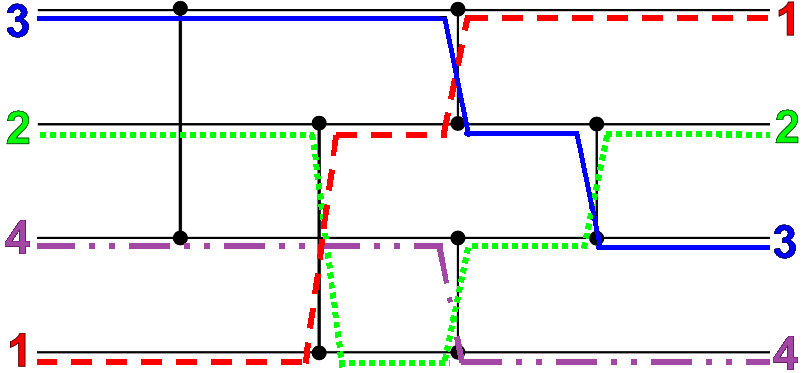
\includegraphics[width=0.4\textwidth]{NetworkTransparent.png} 
	\caption{Voorbeeld van een sorteernetwerk bestaande uit $4$~kanalen en $5$~comparatoren.}
	\label{Werking}
\end{figure}

Om te onderzoeken of een comparator netwerk een sorteernetwerk is, kunnen we gebruik maken van het \textit{nul - \'e\'en principe}. 
Dit principe, zoals beschreven volgens Knuth \cite{Knuth3}, stelt dat om na te gaan of een comparator netwerk met $n$ kanalen een sorteernetwerk is, er enkel nagegaan moet worden dat alle $2^n$ mogelijke sequenties van $n$ nullen en enen gesorteerd worden.
De optimale grootte van een sorteernetwerk met $n$ kanalen is reeds bewezen tot en met $n \leq 10$ (Tabel \ref{tabel1} \cite{sortingNetworksSize2014}).
\begin{table}[h!]
	\centering
	\begin{tabular}{r|c|c|c|c|c|c|c}
	n & 6 & 7 & 8 & 9 & 10 & 11 & 12\\ 
	\hline 
	bovengrens & 12 & 16 & 19 & 25 & 29 & 35 & 39\\ 
	\hline 
	ondergrens & 12 & 16 & 19 & 25& 29 & 33 & 37\\
	\end{tabular} 
	\caption{Minimaal aantal comparatoren bij $6 \leq n \leq 12$ kanalen.}
	\label{tabel1}
\end{table}
%TODO Hard enter?
Voor $n > 10$ zijn er bovengrenzen gekend door zowel concrete voorbeelden als de systematische constructie van Batcher \cite{sortingNetworksApplications}. 
De ondergrenzen werden gevonden door zowel bewijzen als lemma \ref{lemma1} \cite{Voorhis1972}.
\begin{lemma}
	$S(n+1) \geq S(n) + \lceil \log_2(n) \rceil, \forall n \geq 1$\\
	waarbij geldt dat $S(n)$ gelijk is aan het aantal comparatoren in een sorteernetwerk van optimale grootte met $n$ kanalen.
	\label{lemma1}
\end{lemma}

\newcommand*\rfrac[2]{{}^{#1}\!/_{#2}}
\section{Voorgestelde oplossing}\label{VoorgesteldeOplossing}
Om te bewijzen dat een sorteernetwerk $C^n_k$ een sorteernetwerk is van optimale grootte, moeten we bewijzen dat er geen sorteernetwerk $C^n_{k-1}$ bestaat.
Aangezien $n$ kanalen zorgen voor $\frac{n \left(n-1\right)}{2}$ verschillende comparatoren kunnen er $\left(\rfrac{n \left(n-1\right)}{2}\right) ^k$ verschillende netwerken gevormd worden met  $k$ comparatoren.
Voor $9$ kanalen en $24$ comparatoren betekent dit $2.245 \times 10^{37}$ verschillende netwerken.
Deze grote hoeveelheid maakt het overlopen van alle netwerken niet aantrekkelijk.
Om dit aantal te reduceren zullen we gebruik maken van symmetrie\"en waardoor we bepaalde netwerken reeds kunnen verwijderen bij het aanmaken.

We gebruiken de \textit{genereer- en snoei-methode} zoals beschreven door Codish \textit{et al.} (sectie 3, \cite{sortingNetworksSize2014}).
Deze methode heeft een cyclisch verloop waarbij men bij elke cyclus de set $R^n_k$ uitbreidt naar $N^n_{k+1}$ om vervolgens te snoeien en de set $R^n_{k+1}$ te bekomen (Figuur \ref{GenereerSnoei}).
\begin{figure}[!h]
	\centering
	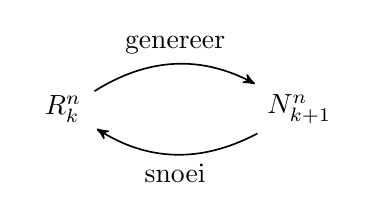
\begin{tikzpicture}[->,>=stealth',shorten >=1pt,auto,node distance=3cm,semithick]
	  \tikzstyle{every state}=[fill=white,draw=none,text=black]

	  \node[state] (A)                    {$R^n_k$};
	  \node[state] (B) [right of=A] {$N^n_{k+1}$};

	  \path (A) edge [bend left] node {genereer} (B)
	  		  (B) edge [bend left] node {snoei} (A);
	\end{tikzpicture}
	\caption{Genereer en snoei principe}
	\label{GenereerSnoei}
\end{figure}
Specifiek zullen we vertrekken van een netwerk zonder comparatoren om te eindigen bij $R^n_k$ bestaande uit \'e\'en sorteernetwerk van optimale grootte.
Bij de genereer-stap zullen we aan elk netwerk van $R^n_k$ alle mogelijke comparatoren toevoegen zodat $|N^n_{k+1}| = |R^n_{k}| \times \frac{n\left(n-1\right)}{2}$.
%TODO aanelkaarpraten zin misschien aanpassen)
Bij de snoei-stap zullen we dan netwerken verwijderen volgens het subsumes principe beschreven in definitie \ref{definitie1}.
\begin{definitie}[Subsumes] %TODO VRAGEN SUBSUMES => TOM NEDERLANDS/ENGELS
	We zeggen ``Comparator netwerk $C^n_{k,a}$ subsumes comparator netwerk $C^n_{k,b}$'' wanneer een permuntatie $\pi$ bestaat zodat ${\pi\left(outputs\left(C_{a}\right)\right) \subseteq outputs\left(C_{b}\right)}$. Dit wordt genoteerd als $ C_{a} \preceq C_{b}$ om aan te duiden dat er een permutatie $\pi$ bestaat zodat $C_{a}\leq_\pi C_{b}$. %TODO Vincent weent om dit te kunnen herzien
	\label{definitie1}
\end{definitie}
\begin{lemma}
	Wanneer voor comparator netwerk $C^n_{k,a}, C^n_{k,b}$ en $C$ geldt dat $ C_{a} \preceq C_{b}$ en er bestaat een sorteernetwerk gevormd door de concatenatie van $C_b$ en $C$ van grootte $m$ dan bestaat er ook een sorteernetwerk gevormd door de concatenatie van $C_a$ en $C'$ van grootte $m$.
	\label{lemma2}
\end{lemma}
Concreet kunnen we de definitie van subsumes en lemma~\ref{lemma2} beschreven door Codish \textit{et al.} gebruiken om in te zien dat we netwerken die gesubsumed worden door andere netwerken kunnen verwijderen\cite{sortingNetworksSize2014}.
Wanneer een set van netwerken een sorteernetwerk bevat, zal het snoeien van deze set resulteren in het bekomen van het sorteernetwerk.
Dit gegeven kan gebruikt worden om de eindigheid van het algoritme in te zien.

Om na te gaan dat er een permutatie $\pi$ bestaat zodat ${\pi\left(Outputs\left(C_{a}\right)\right) \subseteq Outputs\left(C_{b}\right)}$, en dus $C_a \preceq C_{b}$, zouden we alle permutaties kunnen overlopen.
Om deze kostelijke bewerkingen te vermijden en te versnellen, zullen we extra methoden moeten invoeren om sneller beslissingen te maken over het ``subsumen van een ander netwerk''. 
Deze beslissingen kunnen zowel tijdens de genereer-stap als de snoei-stap plaats vinden.

In de volgende subsecties zal de voorgestelde oplossing specifieker beschreven worden.
In subsectie \ref{RepresentatieVanComparatorNetwerken} wordt beschreven hoe effici\"ent de informatie van een comparator netwerk kan worden opgeslagen.
Vervolgens zal in subsectie \ref{Genereren} en \ref{Snoeien} zowel de opbouw van de genereer- en snoei-methode als de extra beslismethoden toegelicht worden.
Bijkomend zullen we een manier geven in subsectie \ref{Parallellisatie} om het proces te parallelliseren zonder al te veel locks.
Tenslotte wordt het geheugengebruik van de implementatie besproken en wordt er manier aangeboden om deze nog verder te beperken.

\subsection{Representatie van comparator netwerken}\label{RepresentatieVanComparatorNetwerken}
Bij de representatie van comparator netwerken moeten we rekening houden met het geheugengebruik en de mogelijkheid om effici\"ente bewerkingen te kunnen uitvoeren.
Concreet zullen we comparatoren voorstellen door een sequentie van bits waarbij twee bits op \'e\'en staan.
Bijvoorbeeld  $ \left[ 0 1 0 0 1 0 \right]$ stelt de comparator $\left(2,5\right)$ voor bij een netwerk van $6$ kanalen.
Om de hoeveelheid overbodige bits te beperken, zullen we bij de \texttt{Java} implementatie gebruik maken van shorts\footnote{In \texttt{Java} bestaat een short uit $16$ bits.}.
Dit is voldoende voor een bewijs tot en met $16$ kanalen.
Buiten de comparatoren worden ook de mogelijke uitvoer van het netwerk bijgehouden.
Aangezien het nul-\'e\'en-principe stelt dat enkel sequenties van nullen en enen getest moeten worden, kunnen we de uitvoer opdelen per aantal enen.
Voor een netwerk zonder comparatoren betekent dit $2^n$ mogelijke uitvoer sequenties.
Dit aantal zal echter dalen naarmate er meer en meer comparatoren worden toegevoegd om uiteindelijk te eindigen met slechts $n$ uitvoer sequenties.
Door de gekozen representatie van invoer en comparatoren kunnen we Code \ref{SwapCompare} gebruiken om de uitvoer van een comparator te bepalen gegeven een bepaalde invoer.
\begin{lstlisting}[caption={swapCompare}, label=SwapCompare]
/**
input - De invoer voor de comparator.
comp - De comparator (bv. 00101)
return - Het resultaat bekomen door de bits van de input om te wisselen afhankelijk van de comparator.
*/
short swapCompare(short input, short comp) {
	int channel1 = 31 - Integer.numberOfLeadingZeros(comp);
	int channel2 = Integer.numberOfTrailingZeros(comp);
	int firstBit = (input >> channel1) & 1;
	int secondBit = (input >> channel2) & 1;
	
	return (firstBit <= secondBit) ? input : (input ^ comp);
}
\end{lstlisting}

In de \texttt{Java} implementatie kiezen we er voor om een comparator netwerk voor te stellen door een tweedimensionale array van shorts, short[][], en laten we de rij van $n$ nullen en $n$ enen  weg.
Een voorbeeld van zo een representatie staat in tabel \ref{tabel2}.
\begin{table}[!h]
	\centering
	\begin{tabular}{r|ccc}
	Comparators & $\left[0011\right]$ & $\left[1010\right]$ & \\ 
	\hline 
	Outputs \'e\'en 1& $\left[0001\right]$ & $\left[0100\right]$ & $\left[0010\right]$ \\ 
	\hline 
	Outputs twee 1'en &$\left[0011\right]$ & $\left[0101\right]$ & $\left[0110\right]$\\ 
	\hline 
	Outputs drie 1'en & $\left[0111\right]$ & $\left[1011\right]$ &  \\ 
	\end{tabular}
	\caption{Representatie $C^4_2$: $(1,2)(2,4)$}
	\label{tabel2}
\end{table}

\subsection{Genereren}\label{Genereren}
\begin{wrapfigure}{r}{0.12\textwidth}
	\vspace{-15pt}
	\begin{subfigure}[b]{0.10\textwidth}
	\centering
    		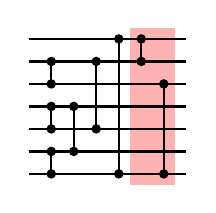
\begin{tikzpicture}
			\def\x{3.5}
			\fill [red!30] (4.5/\x,0.5/\x) -- (6.5/\x,0.5/\x) -- (6.5/\x,7.5/\x) -- (4.5/\x,7.5/\x) -- cycle;
			\foreach \a in {1/\x, 2/\x, 3/\x, 4/\x, 5/\x, 6/\x, 7/\x}
			\draw[thick] (0,\a) -- ++(7/\x,0);
			\foreach \b in {{1/\x,1/\x},{1/\x,2/\x},{1/\x,3/\x},{1/\x,4/\x},{1/\x,5/\x},{1/\x,6/\x},{2/\x,2/\x},{2/\x,4/\x},{3/\x,3/\x},{3/\x,6/\x},{4/\x,1/\x},{4/\x,7/\x},{5/\x,6/\x},{5/\x,7/\x},{6/\x,1/\x},{6/\x,5/\x}}
			\filldraw (\b) circle (1.5 pt);
			\draw[thick] (1/\x,1/\x) -- (1/\x,2/\x);
			\draw[thick] (1/\x,3/\x) -- (1/\x,4/\x);
			\draw[thick] (1/\x,5/\x) -- (1/\x,6/\x);
			\draw[thick] (2/\x,2/\x) -- (2/\x,4/\x);
			\draw[thick] (3/\x,3/\x) -- (3/\x,6/\x);
			\draw[thick] (4/\x,1/\x) -- (4/\x,7/\x);
			\draw[thick] (5/\x,6/\x) -- (5/\x,7/\x);
			\draw[thick] (6/\x,1/\x) -- (6/\x,5/\x);
		\end{tikzpicture}
		\caption{Netwerk 1}
		\label{fig1}
    \end{subfigure}
    \begin{subfigure}[b]{0.10\textwidth}
    \centering
		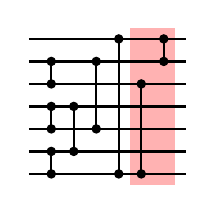
\begin{tikzpicture}
			\def\x{3.5}
			\fill [red!30] (4.5/\x,0.5/\x) -- (6.5/\x,0.5/\x) -- (6.5/\x,7.5/\x) -- (4.5/\x,7.5/\x) -- cycle;
			\foreach \a in {1/\x, 2/\x, 3/\x, 4/\x, 5/\x, 6/\x, 7/\x}
			\draw[thick] (0,\a) -- ++(7/\x,0);
			\foreach \b in {{1/\x,1/\x},{1/\x,2/\x},{1/\x,3/\x},{1/\x,4/\x},{1/\x,5/\x},{1/\x,6/\x},{2/\x,2/\x},{2/\x,4/\x},{3/\x,3/\x},{3/\x,6/\x},{4/\x,1/\x},{4/\x,7/\x},{6/\x,6/\x},{6/\x,7/\x},{5/\x,1/\x},{5/\x,5/\x}}
			\filldraw (\b) circle (1.5 pt);
			\draw[thick] (1/\x,1/\x) -- (1/\x,2/\x);
			\draw[thick] (1/\x,3/\x) -- (1/\x,4/\x);
			\draw[thick] (1/\x,5/\x) -- (1/\x,6/\x);
			\draw[thick] (2/\x,2/\x) -- (2/\x,4/\x);
			\draw[thick] (3/\x,3/\x) -- (3/\x,6/\x);
			\draw[thick] (4/\x,1/\x) -- (4/\x,7/\x);
			\draw[thick] (6/\x,6/\x) -- (6/\x,7/\x);
			\draw[thick] (5/\x,1/\x) -- (5/\x,5/\x);
		\end{tikzpicture}
		\caption{Netwerk 2}
		\label{fig2}
    \end{subfigure}
    \caption{}
    \vspace{-10pt}
\end{wrapfigure}
Bij de genereer-stap itereren we over de set $R^n_k$ en voegen we bij elk netwerk alle mogelijke comparatoren toe.
Een overbodige comparator voor een bepaald comparator netwerk is een comparator die, wanneer toegevoegd aan het comparator netwerk, geen wijziging veroorzaakt in de mogelijke uitvoer.
Wanneer een overbodige comparator wordt toegevoegd aan een comparator netwerk, zal deze gesubsumed worden door een uitbreiding van dat netwerk met een niet overbodige comparator.
Bijgevolg kunnen we deze meteen uit de set $N^n_{k+1}$ verwijderen. 
Om te beslissen of een comparator al dan niet overbodig is, moeten we voor elke mogelijke uitvoer nagaan of deze een wijziging teweegbrengt.
We kunnen dit sneller laten verlopen door eerst te kijken of de comparator al dan niet identiek is met de vorige comparator in het netwerk.

Wanneer twee netwerken, op de volgorde van hun parallelle comparatoren na, gelijk zijn, zoals in figuur \ref{fig1} en \ref{fig2}, zullen deze elkaar subsumen en zal \'e\'en van de twee verwijderd worden.
Dit kan opgevangen worden in de generatie-stap om zo extra werk in de snoei-stap te vermijden.
Bij het toevoegen van een nieuwe comparator $(a,b)$ moet er dan gecontroleerd worden of deze comparator een kanaal gemeenschappelijk heeft met de vorige (Code \ref{TestParallelleComparatoren}).
\begin{lstlisting}[caption={Test op parallelle comparatoren.},label=TestParallelleComparatoren]
(a,b) & vorigeComp != 0
\end{lstlisting}
Wanneer dit niet het geval is en het dus parallelle comparatoren zijn, kunnen we bijvoorbeeld kiezen om het netwerk weg te gooien waarbij de nieuwe comparator kleiner is dan de vorige.

Tenslotte kunnen we, na het toevoegen van de comparator, de nieuwe uitvoer berekenen door de huidig bijgehouden uitvoer als invoer te gebruiken voor de nieuwe comparator.
Om de effici\"entie te verhogen kunnen we bij de omzetting van de uitvoer eerder verkregen informatie gebruiken.
Een comparator is namelijk niet overbodig wanneer er een uitvoer bestaat met een $s$ aantal enen waarvoor geldt dat de comparator deze uitvoer wijzigt.
Deze informatie kan gebruikt worden om bij de omzetting slechts te beginnen bij uitvoer met het aantal enen gelijk aan $s$.
Een algemene structuur van deze code wordt ge\"illustreerd in Code \ref{PseudocodeS}.
\begin{lstlisting}[caption={Pseudocode - optimalisatie via $s$}, label=PseudocodeS]
for(short nieuweComp : comparatoren) {
	int s = vanafAantalEnenWijzigt(netwerk, nieuweComp);
	if(s != -1) {
		voegToeAanNetwerk(netwerk, nieuweComp, s)
	}
}
\end{lstlisting}

\subsection{Snoeien}\label{Snoeien}
Bij de snoei-stap lopen we over de set $N^n_{k+1}$ en verwijderen we alle comparator netwerken die gesubsumed worden door een ander comparator netwerk in de resterende set.
Om het aflopen van alle permutaties te vermijden, en sneller te beslissen of $C_a \preceq C_b$ met $C_a$ en $C_b$ twee comparator netwerken, voeren we enkele methoden in.
Zo gebruiken we onder meer lemma \ref{lemma3} en lemma \ref{lemma4}, beschreven in 
\begin{small}
\textsc{Twenty-Five Comparators is Optimal when Sorting Nine Inputs (and Twenty-Nine for Ten)}
\end{small}
\cite{sortingNetworksSize2014}.

Bij $9$ kanalen wordt lemma \ref{lemma3} $1.07666 \times 10^{13}$ keer nagegaan waarbij $1.05438 \times 10^{13}$ keer een beslissing genomen wordt.
\begin{lemma}
	Wanneer de uitvoerverzameling bij $C_a$ met $x$ enen ($1 \leq x \leq n$) groter is dan bij $C_b$ weten we dat $C_a \npreceq C_b$ met $C_a$ en $C_b$ twee comparator netwerken.
\label{lemma3}
\end{lemma}
Voor lemma \ref{lemma4} introduceren we extra informatie over het comparator netwerk, namelijk $w\left(C_a, x, k\right)$ waarbij ${x \in \{0,1\}}$ en $0\leq k \leq n$.
Dit representeert de set van posities $i$ waarvoor er een uitvoer bestaat in $C_a$ met $k$ enen waarvoor geldt dat op de $i^{de}$ positie van deze uitvoer een $x$ voorkomt.
Om effici\"ent operaties te kunnen uitvoeren, zullen we de posities voorstellen door middel van een bit representatie.
Zo zal bijvoorbeeld $w\left(C_a, 1, 2\right) = 0110$ inhouden dat er bij de uitvoerverzameling met twee enen minstens \'e\'en uitvoer bestaat met een $1$ op de $2^{de}$ positie, \'e\'en met een $1$ op de $3^{de}$ positie en geen enkel met een $1$ op positie $1$ of $4$.
Deze informatie voegen we bij elk netwerk toe in de vorm van een array van shorts, $w^*$.
Aangezien er geen uitvoer wordt bijgehouden met $0$ enen en $n$ enen zullen we enkel voor $k \geq 1 $ en $k \leq n-1$ zowel $w$ als de grootte van $w$ bijhouden.
Dit vereist voor elk dan vier opeenvolgende indices in $w^*$, zoals te zien in figuur \ref{tabel3}.
Deze informatie slaan we voor elke $k$ op vanaf index\footnote{In \texttt{Java} begint een array met index $0$.} $(k-1) \times 4$.
Wanneer we bij het toevoegen van een comparator $w^*$ herberekenen, kunnen we net zoals bij de omzetting van de uitvoer slechts beginnen bij de uitvoerverzameling met het aantal enen gelijk aan $s$.
%\begin{table}[!h]
%	\centering
%	\begin{tabu}{|[1.2pt]l|[1.2pt]c|[1.2pt]c|[1.2pt]c|[1.2pt]}
%	\tabucline[1.2pt]{-}
%	$w\left(C_a, 0, 1\right)$ & $|w\left(C_a, 0, 1\right)|$  & $w\left(C_a, 1, 1\right)$ & $|w\left(C_a, 1, 1\right)|$\\ 
%	\tabucline[1.2pt]{-}
%	\end{tabu} 
%	\caption{De inhoud van $w$ op indices $0-3$ voor \'e\'en 1.}
%	\label{tabel3} 
%\end{table}
\begin{figure}[!h]
	\centering
	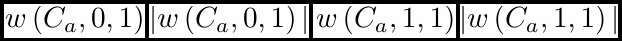
\includegraphics[width = 0.45\textwidth]{Tabel3_OpbouwW.png}
	\caption{De inhoud van $w^*$ op indices $0-3$ voor $k = 1$.}
	\label{tabel3} 
\end{figure}

\begin{lemma}
	Wanneer voor een comparator netwerk $C_a$ en $C_b$ met $n$ kanalen geldt dat $|w\left(C_a, x, k\right)| > |w\left(C_b, x, k\right)|$ voor $x \in \{0,1\}$ en $0 \leq k \leq n$ dan $C_a \npreceq C_b$.
	\label{lemma4}
\end{lemma}
De methode van lemma \ref{lemma4} wordt bij $9$ kanalen ${2.22803 \times 10^{11}}$ keer uitgevoerd waarbij $2.05631 \times 10^{11}$ keer een beslissing genomen wordt.
Dit lemma voorkomt, net zoals lemma \ref{lemma3}, dat er permutaties getest moeten worden.

Als beide lemma's geen uitsluiting bieden, zullen we permutaties moeten nagaan.
Een na\"ieve methode zou zijn om alle $n!$ permutaties te overlopen.
In de plaats daarvan zullen we enkel permutaties afgaan die voldoen aan lemma \ref{lemma5}\cite{sortingNetworksSize2014}.
\begin{lemma}
	${C_a \preceq C_b  \Rightarrow \pi\left(Outputs\left(C_{a}\right)\right) \subseteq Outputs\left(C_{b}\right)} \Rightarrow \pi\left(w\left(C_a, x, k\right)\right) \subseteq w\left(C_b, x, k\right)$,
	${\forall x \in \{0,1\}, \forall k \in \{1..n\}}$.
\label{lemma5}
\end{lemma}

Om de mogelijke permutaties bij te houden zullen we gebruik maken van een voorstelling die te zien is in tabel \ref{tabel4}.
De waarden in een kolom stellen alle mogelijke posities voor die op die plaats kunnen voorkomen.
Wanneer we tabel  \ref{tabel4} gebruiken om de mogelijke permutaties weer te geven dan zullen we permutatie $4321$ en $1324$  bekomen, waarbij $4321$ een eenheidspermutatie zal voorstellen.
Bij het begin van het algoritme zullen we starten met tabel \ref{tabel5}, deze laat alle $n!$ permutaties toe.
Hierna gebruiken we lemma \ref{lemma5} om posities uit de kolommen te verwijderen.
\begin{table}[!h]
	\centering
	\begin{tabular}{|c|c|c|c|}
	\hline
	1 & 2 & 2 & 1 \\ 
	2 & 3 &  &  \\ 
	4 &  &  &  \\ 
	\hline 
	\end{tabular}
	\caption{Een voorbeeld van een permutatietabel voor 4 kanalen.}
	\label{tabel4}
\end{table}
\begin{table}[!h]
	\centering
	\begin{tabular}{|c|c|c|c|}
	\hline
	1 & 1 & 1 & 1 \\ 
	2 & 2 & 2 & 2\\ 
	3 & 3 & 3 & 3 \\
	4 & 4 & 4 & 4\\ 
	\hline 
	\end{tabular}
	\caption{Een permutatietabel in het begin van het algoritme voor 4 kanalen.}
\label{tabel5}
\end{table}

We weten namelijk dat als \[{\pi\left(outputs\left(C_a\right)\right) \subseteq outputs\left(C_b\right)}\] er bij de gepermuteerde outputs enkel een $1$ kan komen op de plaats waar dit bij $C_b$ ook het geval is.
Op de plaats waar $C_b$ een $0$ heeft, kunnen dus enkel de posities komen waar $C_a$ een $0$ heeft.
Nemen we bijvoorbeeld $w\left(C_a,1,1\right) = 0101$ en ${w\left(C_b,1,1\right)=0110}$ dan kunnen we tabel \ref{tabel5} reduceren tot tabel \ref{tabel6}.
We kunnen voor $w\left(C_a, x, k\right)$ deze methode doortrekken voor elke $1 \leq k \leq n$ en voor zowel $x = 0$ als $x = 1$.
Wanneer we elke kolom bijhouden door een bit representatie kunnen we gemakkelijk de doorsnede van de mogelijke posities nemen na elke berekening voor een bepaalde $k$ en $x$ door middel van de $\&$-operatie. 
\begin{table}[!h]
	\centering
	\begin{tabular}{|c|c|c|c|}
	\hline
	2 & 1 & 1 & 2 \\ 
	4 & 2 & 2 & 4\\ 
	 & 3 & 3 &  \\
	 & 4 & 4 & \\ 
	\hline 
	\end{tabular}
	\caption{Een permutatietabel voor 4 kanalen.}
	\label{tabel6}
\end{table}

Wanneer tijdens het algoritme een kolom leeg zou komen te staan, kunnen we het algoritme stopzetten.
Dit betekent namelijk dat er geen enkele permutatie bestaat die niet door lemma \ref{lemma5} wordt afgekeurd.
Mocht op het einde een kolom \'e\'en element hebben, mogen we dit element uit alle andere kolommen verwijderen.
We kunnen nadien ook nog nagaan of alle elementen minstens \'e\'enmaal voorkomen in de hele tabel.
Tot slot gebruiken we de overblijvende permutatietabel om onze mogelijke permutaties, die aan lemma \ref{lemma5} voldoen, na te gaan. 
Dit kan onder andere door middel van een recursieve methode.

\subsection{Parallellisatie}\label{Parallellisatie}
\begin{wrapfigure}{l}{0.20\textwidth}
	\centering
	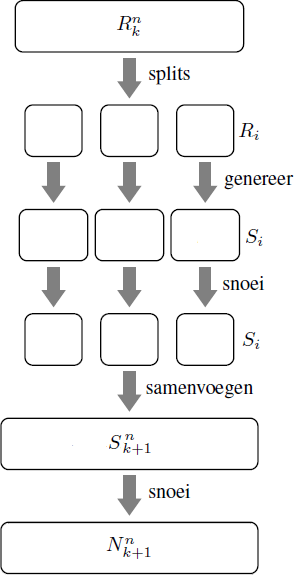
\includegraphics[scale=0.5]{Gen_Prune_Opbouw.png}
	\caption{Opbouw parallelle genereer \& snoei}
	\label{opbouwGenPrune}
\end{wrapfigure}
Om het algoritme te laten functioneren met meerdere processoren, zullen we enkele aanpassingen doorvoeren.
Bij de overgang van $R^n_k$ naar $N^n_{k+1}$ zal elke thread een aantal netwerken uit $R^n_k$ nemen, in ons geval $256$, hierop de genereer-stap uitvoeren en vervolgens binnen de resulterende set de snoei-stap uitvoeren.
Op dat moment beschikt elke thread over een set van netwerken met $k+1$ comparatoren waarop de snoei-stap nog moet worden uitgevoerd ten opzichte van alle andere sets.
Elke thread zal vervolgens zijn set in een gedeelde lijst $S^n_{k+1}$ in het centraal geheugen plaatsen.
Om deze operatie zo effici\"ent mogelijk te maken, vermijden we zowel locks als het moeten vergroten van de lijst. 
Daarom zullen we in het begin van de cyclus zorgen dat deze lijst groot genoeg is en gebruik maken van een variabele die bijhoudt op welke index een volgend netwerk moet worden bijgevoegd.
In onze \texttt{Java} implementatie zullen we voor deze variabele een \texttt{AtomicInteger} gebruiken, deze variabele garandeert een atomische \texttt{getAndIncrement(int)} functie.
Een thread kan deze functie gebruiken om voldoende plaats in de lijst op te eisen voor zijn set door de grootte van zijn set mee te geven als parameter.

Na het toevoegen aan de gedeelde lijst volgt de snoei-stap. Hier zal elke thread subsumes moeten nagaan tussen alle netwerken in zijn set en elk ander reeds toegevoegd netwerk.
Door het (hopelijk) vele verwijderen van netwerken ontstaan er veel opeenvolgende lege plaatsen in de lijst\footnote{Bij de \texttt{Java} implementatie zullen we verwijderen via  ``${= null}$''.}.
Hierdoor zal het algoritme vaak overbodig het netwerk opvragen.
Om dit aantal, dat groter wordt naarmate het aantal kanalen stijgt, te verminderen, introduceren we een manier om deze opeenvolgende lege indices over te slaan. 
Telkens wanneer een lege index wordt gedetecteerd door een thread zal deze het aantal opeenvolgende lege indices tellen en dit aantal opslaan op de eerste lege plaats in deze reeks.
Dit getal stelt dus het aantal opeenvolgende lege plaatsen voor na die index.
Wanneer een thread dan dit getal tegenkomt, weten we exact hoeveel indices de thread kan overslaan.
%TODO Big O ??
%TODO ZIe pagina 4 in paper => definitie 2: Observe that ......

\subsection{Geheugen}\label{Geheugen}
Door het grote aantal netwerken is het testen op subsumes en de effici\"entie van de datastructuren van groot belang. In figuur \ref{netwerkVerloop9kanalen} zien we dat dit aantal voor $9$ kanalen kan oplopen tot meer dan $900000$ netwerken. Bij het stijgen van het aantal kanalen wordt dan ook het geheugenbeheer des te belangrijker.
\begin{figure}[!h]
	\centering
	\begin{tikzpicture}
		\begin{axis} [
			xlabel={Aantal comparatoren},
			ylabel={Aantal netwerken},
			ymode = log,
			log basis y = 10,
			legend pos = north west,
			ymajorgrids=true]
		\addplot [only marks, green] file {netwerkVerloop7kanalen.dat};
		\addplot [only marks, blue] file {netwerkVerloop8kanalen.dat};
		\addplot [only marks, red] file {netwerkVerloop9kanalen.dat};
		\addplot [only marks, cyan] file {netwerkVerloop10kanalen.dat};
		\addplot [smooth, green] file {netwerkVerloop7kanalen.dat};
		\addplot [smooth, blue] file {netwerkVerloop8kanalen.dat};
		\addplot [smooth, red] file {netwerkVerloop9kanalen.dat};
		\addplot [smooth, cyan] file {netwerkVerloop10kanalen.dat};
		\legend{7 kanalen, 8 kanalen, 9 kanalen, 10 kanalen\footnotemark};
		\end{axis}
	\end{tikzpicture}
	\caption{Aantal resterende netwerken na het uitvoeren van genereer en snoei bij toevoegen van de $k^{de}$ comparator.}
	\label{netwerkVerloop9kanalen}
\end{figure}
\footnotetext{Voor $10$ kanalen is het aantal netwerken berekend tot en met comparator $13$.} %TODO UPDATE??
%TODO CHECK VERLEDEN <=> TTTijd

In \texttt{Java} hebben we het voordeel dat we niet expliciet aan geheugenbeheer moeten doen.
We gaan anderzijds wel enkele maatregelen nemen om de vereiste hoeveelheid geheugen te verlagen.
E\'en van de mogelijke plaatsen waar we dit kunnen doen, is bij de representatie van een netwerk.
Wanneer een comparator aan een netwerk wordt toegevoegd is het mogelijk dat een lijst van uitvoer sequenties met $s$ enen ongewijzigd blijft.
Om te vermijden dat we hierdoor meerdere malen dezelfde lijst in het geheugen hebben, zullen we een referentie doorgeven van deze lijst en slechts een nieuwe lijst gebruiken wanneer de lijst gewijzigd wordt.
Aangezien bij \texttt{Java} een tweedimensionale lijst wordt aanzien als een lijst van referenties naar andere lijsten kan de oude referentie gemakkelijk herbruikt worden. 

Een andere plaats is bij de parallellisatie, hier daalt de hoeveelheid geheugen doordat een thread enerzijds zal snoeien binnen zijn set alvorens de set toe te voegen aan de gedeelde lijst en anderzijds doordat de genereer- en snoei-stap door elkaar worden uitgevoerd.

Onze \texttt{Java} implementatie gebruikte bij de uitvoering voor $8$ en $9$ kanalen respectievelijk $208$MB en $3951$MB.
Deze hoeveelheid kan verschillen naargelang de frequentie waarbij de \texttt{Java Virtual Machine} de \textit{Garbage Collection} uitvoert.
Voor minder dan $8$ kanalen was het geheugen verbruik verwaarloosbaar klein.

\section{Evaluatie}\label{Evaluatie}
Het beschreven algoritme, ge\"implementeerd in \texttt{Java}, vindt voor $9$ kanalen reeds na $3$ uur en $25$ minuten een oplossing met $25$ comparatoren die gevisualiseerd wordt in figuur~\ref{Sorteernetwerk9kanalen}.
Dit bevestigt wat reeds geweten was \cite{sortingNetworksSize2014}.
\begin{figure}[!h]
\centering
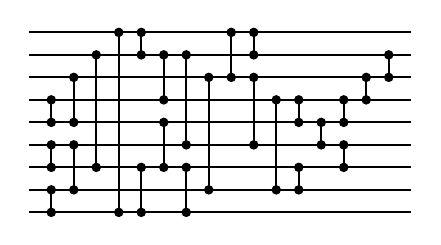
\begin{tikzpicture}
\def\x{3.5}
\foreach \a in {1/\x, 2/\x, 3/\x, 4/\x, 5/\x, 6/\x, 7/\x, 8/\x, 9/\x}
  \draw[thick] (0,\a) -- ++(17/\x,0);
\foreach \b in {{1/\x,1/\x},{1/\x,2/\x},{1/\x,3/\x},{1/\x,4/\x},{1/\x,5/\x},{1/\x,6/\x},{2/\x,2/\x},{2/\x,4/\x},{2/\x,5/\x},{2/\x,7/\x},{3/\x,3/\x},{3/\x,8/\x},{4/\x,1/\x},{4/\x,9/\x},{5/\x,8/\x},{5/\x,9/\x},{5/\x,1/\x},{5/\x,3/\x},{6/\x,3/\x},{6/\x,5/\x},{7/\x,1/\x},{7/\x,3/\x},{6/\x,6/\x},{6/\x,8/\x},{7/\x,4/\x},{7/\x,8/\x},{8/\x,2/\x},{8/\x,7/\x},{9/\x,7/\x},{9/\x,9/\x},{10/\x,8/\x},{10/\x,9/\x},{10/\x,4/\x},{10/\x,7/\x},{11/\x,2/\x},{11/\x,6/\x}, {12/\x,2/\x},{12/\x,3/\x},{12/\x,5/\x},{12/\x,6/\x},{13/\x,4/\x},{13/\x,5/\x},{14/\x,3/\x},{14/\x,4/\x},{14/\x,5/\x},{14/\x,6/\x},{15/\x,6/\x},{15/\x,7/\x},{16/\x,7/\x},{16/\x,8/\x}}
  \filldraw (\b) circle (1.5 pt);
\draw[thick] (1/\x,1/\x) -- (1/\x,2/\x);
\draw[thick] (1/\x,3/\x) -- (1/\x,4/\x);
\draw[thick] (1/\x,5/\x) -- (1/\x,6/\x);
\draw[thick] (2/\x,2/\x) -- (2/\x,4/\x);
\draw[thick] (2/\x,5/\x) -- (2/\x,7/\x);
\draw[thick] (3/\x,3/\x) -- (3/\x,8/\x);
\draw[thick] (4/\x,1/\x) -- (4/\x,9/\x);
\draw[thick] (5/\x,8/\x) -- (5/\x,9/\x);
\draw[thick] (5/\x,1/\x) -- (5/\x,3/\x);
\draw[thick] (6/\x,3/\x) -- (6/\x,5/\x);
\draw[thick] (7/\x,1/\x) -- (7/\x,3/\x);
\draw[thick] (6/\x,6/\x) -- (6/\x,8/\x);
\draw[thick] (7/\x,4/\x) -- (7/\x,8/\x);
\draw[thick] (8/\x,2/\x) -- (8/\x,7/\x);
\draw[thick] (9/\x,7/\x) -- (9/\x,9/\x);
\draw[thick] (10/\x,8/\x) -- (10/\x,9/\x);
\draw[thick] (10/\x,4/\x) -- (10/\x,7/\x);
\draw[thick] (11/\x,2/\x) -- (11/\x,6/\x);
\draw[thick] (12/\x,2/\x) -- (12/\x,3/\x);
\draw[thick] (12/\x,5/\x) -- (12/\x,6/\x);
\draw[thick] (13/\x,4/\x) -- (13/\x,5/\x);
\draw[thick] (14/\x,3/\x) -- (14/\x,4/\x);
\draw[thick] (14/\x,5/\x) -- (14/\x,6/\x);
\draw[thick] (15/\x,6/\x) -- (15/\x,7/\x);
\draw[thick] (16/\x,7/\x) -- (16/\x,8/\x);
\end{tikzpicture}
\caption{Sorteernetwerk 9 kanalen, 25 comparatoren}
\label{Sorteernetwerk9kanalen}
\end{figure}

De tijdsmetingen voor het vinden van een sorteernetwerk van optimale grootte van $5$ tot en met $9$ kanalen zijn te zien op figuur \ref{Tijdsresultaten}.
Op deze figuur is ook de tijdsmeting van eerder werk te zien, ongeveer $12$ dagen $17$ uur en $58$ minuten\cite{sortingNetworksSize2014}.
De bekomen resultaten van dit werk zijn afkomstig van het uitvoeren op \'e\'en node bestaande uit twee $12$-core ``Haswell'' Xeon E$5$-$2680$v$3$ processoren ($2.5$GHz, $30$MB level $3$ cache met $64$GB RAM) op de rekeninfrastructuur van het Vlaamse Supercomputer Centrum.
\begin{figure}[!h]
\centering
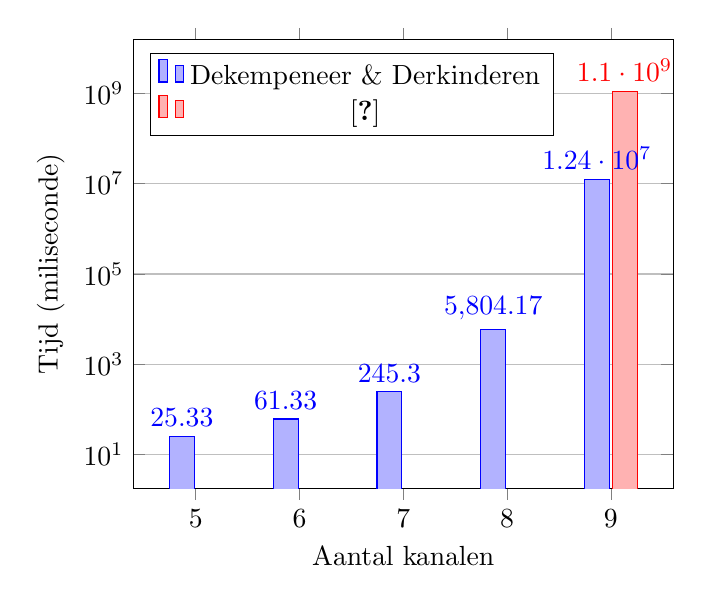
\begin{tikzpicture} 
	\begin{axis}[
		ylabel = Tijd (miliseconde),
		xlabel = Aantal kanalen,
		enlargelimits=0.15,
		ybar=1pt,
		ymode = log,
		log basis y = 10,
		bar width=9pt,
		nodes near coords,
		point meta=10^y,
		ymajorgrids = true,
		legend pos = north west
		]
\addplot
	coordinates {(5, 25.331106) (6, 61.339344) (7, 245.313463) (8, 5804.849367) (9, 12366987.991024)};	
\addplot
	coordinates {(9, 1101480000)};
\legend{Dekempeneer \& Derkinderen, \cite{sortingNetworksSize2014}};
\end{axis}
\end{tikzpicture}
\caption{Tijdsmetingen voor uitvoer bij $5$ tot en met $9$ kanalen.}
\label{Tijdsresultaten}
\end{figure}

\subsection{Benadering 10 en 11 kanalen}
De uitvoering van het programma voor $10$ kanalen is na $299$~uur\footnote{$12$ dagen en $11$ uur} stopgezet. %TODO Aanpassen naar het effectieve
De tussentijdse resultaten met betrekking tot de uitvoeringstijd zijn te zien in figuur \ref{tijdverloop10kanalen} en met betrekking tot het aantal netwerken zijn te zien in figuur \ref{netwerkVerloop9kanalen}.
Voor 10, en dus ook voor 11, kanalen is de \texttt{Java} implementatie met de gebruikte hardware onvoldoende om resultaten binnen een redelijk tijdsbestek te bekomen.
Gebaseerd op figuur \ref{tijdverloop10kanalen} schatten we dat voor $10$ kanalen meer dan $1500$ dagen\footnote{Berekend op basis van een polynomiaal verloop van graad $11$.} vereist zijn. 
\begin{figure}[!h]
\centering
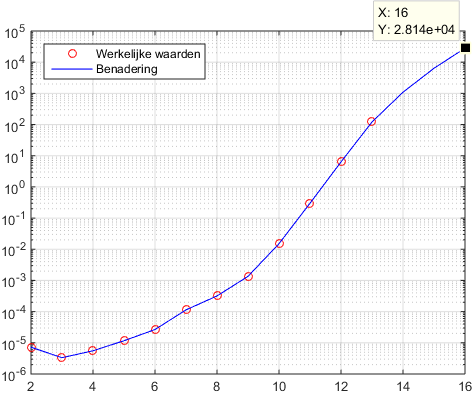
\includegraphics[width = 0.49\textwidth]{Benadering10_paper.png}
\caption{Tijdsverloop $10$ kanalen tot en met de  $13^{de}$ comparator en benadering van tijdsverloop tot en met de $16^{de}$ comparator.}
\label{tijdverloop10kanalen}
\end{figure}

\subsection{Profilering}
Via een profilering, zoals in figuur \ref{ProfileTime9}, kunnen we de bottleneck vaststellen met als doel de uitvoeringstijd te verbeteren.
In dit profiel zien we dat de snoei-methode, de prune-methode in de figuur, duidelijk de bottleneck is.
In deze methode wordt er door een thread voor elk netwerk in de gedeelde lijst subsumes uitgevoerd met elk netwerk in zijn eigen lijst, zoals beschreven in sectie \ref{Parallellisatie}.
Wanneer we de uitvoeringstijd willen verbeteren, kunnen we enerzijds proberen deze prune methode te voorkomen zoals bijvoorbeeld in de genereer-stap en anderzijds door deze prune-methode effici\"enter te maken.
Hier kan bijvoorbeeld onderzoek gedaan worden naar of men al dan niet onder een bepaalde voorwaarde netwerken van de eigen lijst kan overslaan.
\begin{figure}[!h]
\centering
\vspace{10pt}
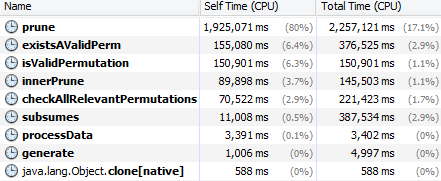
\includegraphics[width=0.49\textwidth]{Profile_Time_9.png}
\caption{Profile van een parti\"ele uitvoering voor $9$ kanalen.} %TODO
\label{ProfileTime9}
\end{figure}

\subsection{Beslissingen}
Door de genereer- en snoei-aanpak mag het totaal aantal te overlopen netwerken dan wel gedaald zijn, de hoeveelheid beslissingen dat er genomen moeten worden blijft nog steeds hoog zoals te zien in figuur \ref{AantalBeslissingen9Kanalen}.
In deze figuur zien we dat de meeste beslissingen genomen worden tijdens het snoeien.
Er moet echter wel een onderscheid gemaakt worden in het soort van beslissingen.
De beslissingen genomen in de genereer-stap zijn beslissingen die het genereren van een netwerk voorkomen en zijn gebaseerd op redundante comparatoren.
Deze beslissingen zorgen voor minder netwerken in de gedeelde lijst en dus voor zowel minder snoei-operaties als geheugenverbruik.

De beslissingen genomen in de snoei-stap daarentegen, zijn beslissingen die enkel voorkomen dat er permutaties moeten worden opgebouwd om na te gaan of $C_a \preceq C_b$ geldt.
Deze zorgen er dus niet voor dat een netwerk uit de gedeelde lijst verdwijnt, enkel dat er niet al te veel tijd gespendeerd wordt aan het onnodig nagaan van permutaties.
Hier wordt onder meer lemma~\ref{lemma3} en lemma~\ref{lemma4} gebruikt.

Vervolgens zijn er nog de beslissingen die genomen worden tijdens de opbouw van de mogelijke permutaties en tijdens het aflopen van deze permutaties.
Tijdens de opbouw gebeurt deze beslissing wanneer er geen geschikte permutatie bestaat doordat de permutatietabel een lege kolom bevat.

\begin{figure}[!h]
\centering
      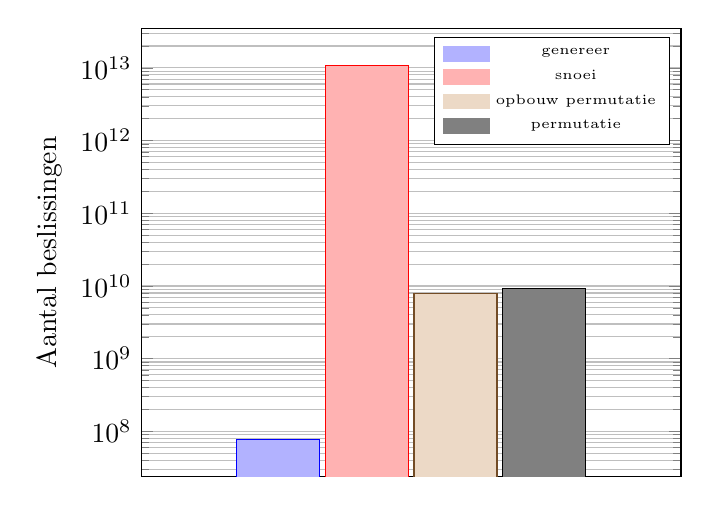
\begin{tikzpicture}
          \begin{axis}[
              ybar,
              ymode = log,
			log basis y = 10,
              ymajorgrids,
              yminorgrids,
              bar width=30pt,
              ylabel=Aantal beslissingen,
              xticklabels={},
              xtick=\empty,
              nodes near coords align={vertical},
			legend image code/.code={ \draw[#1, draw=none] (0cm,-0.1cm) rectangle (0.6cm,0.1cm);},              
              legend style={font=\tiny}
              ]

              \addplot+[error bars/.cd, y dir=both, y explicit] coordinates{ (1,78145401)};
              \addplot+[error bars/.cd, y dir=both, y explicit] coordinates{ (1,10749500000000)};
              \addplot+[error bars/.cd, y dir=both, y explicit] coordinates{ (1,7815523091)};
              \addplot+[error bars/.cd, y dir=both, y explicit] coordinates{ (1,9357151347)};
             \legend{genereer,snoei,opbouw permutatie,permutatie}
          \end{axis}
      \end{tikzpicture}
\caption{Aantal beslissingen bij een uitvoer voor $9$ kanalen.}
\label{AantalBeslissingen9Kanalen}
\end{figure}

\section{Conclusies}
Onze implementatie van de genereer- en snoei-aanpak van Codish \textit{et al} zorgde voor een bewijs voor $9$ kanalen na $3$~uur en $26$~min, een versnelling ten opzichte van de eerdere $305$~uur.
Het is echter niet snel genoeg voor een bewijs van $10$ kanalen, deze zou bij benadering meer dan $1500$ dagen duren.
Bijgevolg blijft het bewijs voor het sorteernetwerk van optimale grootte voor $11$ kanalen het volgende open probleem.
Er zou nog extra werk geleverd kunnen worden omtrent het effici\"ent overlopen van alle comparator netwerken alsook het bruikbaar maken voor meerdere nodes.

\section*{Erkenning}
Graag willen we Professor Dr. Ir. Tom Schrijvers bedanken voor zijn begeleiding doorheen dit onderzoek.\\
De rekeninfrastructuur en dienstverlening gebruikt in dit werk, werd voorzien door het VSC (Vlaams Supercomputer Centrum), gefinancierd door het FWO en de Vlaamse regering - departement EWI.
Bijgevolg willen we de onderzoeksgroep DTAI bedanken voor de aangeboden credits voor deze rekeninfrastructuur.

\bibliographystyle{named}
\bibliography{SortingNetworks}

\end{document}

